The state estimation of a vehicle sits at the junction of vehicle dynamics and control theory. Both knowledge of the dynamics of a race car and the algorithms to model their physics in equations and software is required to design a successful solution. Therefore, we explore the fundamentals of vehicle dynamics, estimation algorithms and sensor failure detection in this chapter.

Throughout this thesis, the conventions of ISO 8855~\cite{ISO.2011} will be used, which assumes a right-handed coordinate system. The vehicle coordinate system uses an upward $z$-axis with a forward $x$-axis and a leftward $y$-axis, while the earth-fixed coordinate system uses an upward $z$-axis with an eastward $x$-axis and a northward $y$-axis. The vehicle's\gls{cog} is used as origin/reference point of the vehicle coordinate system. In case of mixed coordinate systems, left-superscript will be used to denote the reference frame (e.g., $\prescript{V}{}{x}$ for vehicle coordinates, $\prescript{E}{}{x}$ for earth-fixed coordinates).

\section{Rigid Body Kinematics}
The fundamental laws of mechanics apply to race cars as they do to any other body. These laws relate, among others, the body's linear and angular position and its time derivatives, resulting in translational and rotational changes. Their three-dimensional vector definitions are shown in equations \ref{eq:linear-quantities} and \ref{eq:angular-quantities}. To simplify the equations, a rigid body is assumed. This means, that deformations which occur in the vehicle during dynamic maneuvers are negligibly small or vanish. Therefore, points on the body maintain the same distance relative to each other at all times. Furthermore, a two-dimensional motion in the road plane can be assumed in many cases because the effects vertical dynamics are negligible. The simplified equations for that case will also be shown.

\begin{subequations}\label{eq:linear-quantities}
\begin{alignat}{2}%
p &= \begin{bmatrix}x, y, z\end{bmatrix}^T \\%
v &= \begin{bmatrix}v_x, v_y, v_z\end{bmatrix}^T \\%
a &= \begin{bmatrix}a_x, a_y, a_z\end{bmatrix}^T%
\end{alignat}
\end{subequations}
\begin{subequations}\label{eq:angular-quantities}
\begin{alignat}{2}%
\varphi &= \begin{bmatrix}\phi, \theta, \psi\end{bmatrix}^T \\%
\omega &= \begin{bmatrix}\dot{\phi}, \dot{\theta}, \dot{\psi}\end{bmatrix}^T \\%
\alpha &= \begin{bmatrix}\ddot{\phi}, \ddot{\theta}, \ddot{\psi}\end{bmatrix}^T%
\end{alignat}
\end{subequations}

The linear displacement $p$ of a body describes its position relative to the origin of its reference frame. It comprises a longitudinal component along the $x$-axis, a lateral component along the $y$-axis and a vertical component along the $z$-axis. Its first time derivative $v = \frac{dr}{dt}$ and second time derivative $a = \frac{d^2r}{dt^2}$ are the body's linear velocity and acceleration, respectively. \\ The angular orientation $\varphi$ of a body describes its rotation in the reference frame. It can be described by the roll angle $\phi$ around the $x$-axis, the pitch angle $\theta$ around the $y$-axis and the yaw angle, or heading, $\psi$ around the $z$-axis. The angular velocity $\omega$ and acceleration $\alpha$ describe the element-wise time derivatives of these angles. Talking about $p$ and $\varphi$ only makes sense in earth-fixed coordinates.


\subsection{Transformation of Linear Velocities}
All points on a rigid body experience the same angular velocity, i.e. $\omega^A = \omega^B$ for any two points $A, B$ on that body at all times. However, these two points will generally not have the same linear velocity vector, since it is affected by their location $r$ relative to the \gls{cog}. Only when $\omega = \mathbb{0}$, the linear velocity is equal for all points on the body, i.e. $v^A = v^B$. If there is a non-zero angular velocity, equation \ref{eq:offcenter-velocity-3d} holds for any point $P$, assuming the velocity at the \gls{cog} is known (the expanded form can be found in Appendix \ref{sec:appendix-transformation-linvel}).

% For SFII transformation
\begin{equation}\label{eq:offcenter-velocity-3d}%
v^P = v^{CG} + \omega \times r^P%
\end{equation}

This becomes easier to visualize when regarding the two-dimensional case, where $v_z$, $\dot{\phi}$ and $\dot{\theta}$ are disregarded, as shown in equation \ref{eq:offcenter-velocity-2d}.

\begin{equation}\label{eq:offcenter-velocity-2d}%
v^P%
= \begin{bmatrix}v_x^{CG} \\ v_y^{CG} \\ 0\end{bmatrix} + \begin{bmatrix}0 \\ 0 \\ \dot{\psi}\end{bmatrix} \times \begin{bmatrix}r_x \\ r_y \\ r_z\end{bmatrix}%
= \begin{bmatrix}v_x^{CG} \\ v_y^{CG} \\ 0\end{bmatrix} + \begin{bmatrix}-\dot{\psi} \cdot r_y \\ \dot{\psi} \cdot r_x \\ 0\end{bmatrix}%
 \end{equation}

Let us regard the example scenario shown in figure \ref{fig:offcenter-velocity}, where the vehicle has a positive yaw rate and the \gls{cog} is moving forward and to the left. Point $A$ is at the front left ($r_x > 0$, $r_y > 0$), while point $B$ is at the rear right ($r_x < 0$, $r_y < 0$). Since $r$ is defined relative to the \gls{cog}, its position is $\mathbb{0}$. Due to the positive yaw rate, $A$ experiences a higher $v_y$ but lower $v_x$ than the \gls{cog}. $B$, on the other hand, experiences a higher $v_x$ but lower $v_y$ than the \gls{cog}. If the yaw rate were zero, all points would experience the same linear velocity.

\begin{figure}
	\centering
	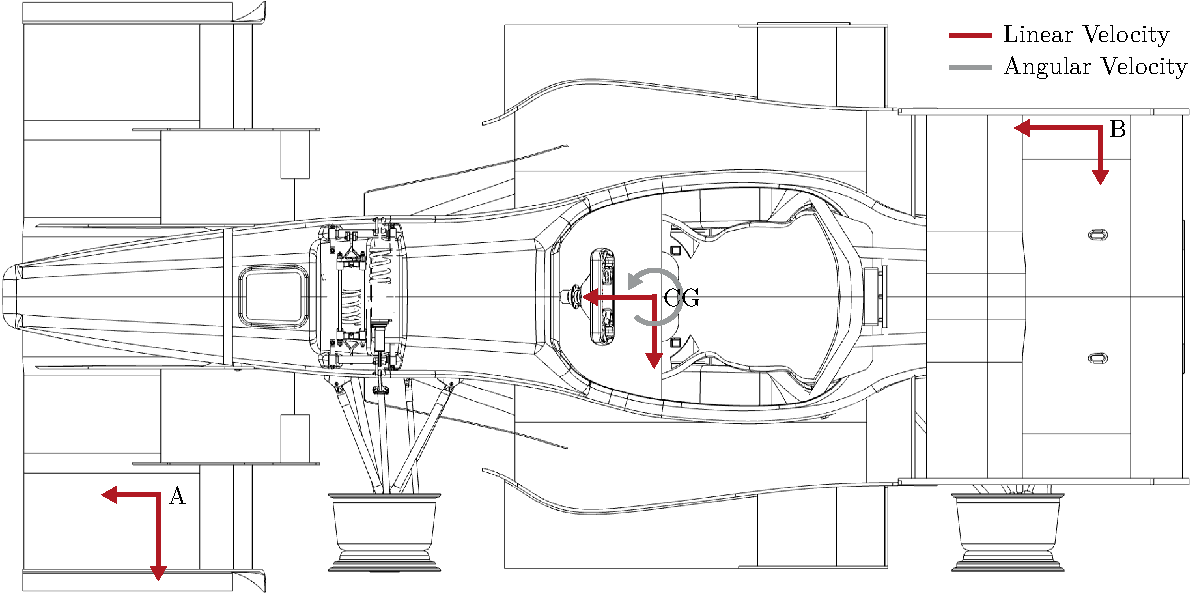
\includegraphics[width=\textwidth]{offcenter_velocity}%
	\caption{Experienced velocities at off-center points}
	\label{fig:offcenter-velocity}
\end{figure}


\subsection{Transformation of Linear Accelerations}
Like the angular velocity, the angular acceleration is the same at every point on a rigid body, i.e. $\alpha^A = \alpha^B$ for any two points $A, B$ on that body. However, these two points will generally not experience the same linear acceleration. Only if the rotational motion components $\omega$ and $\alpha$ are $\mathbb{0}$, the linear acceleration is equal for all points on the body, i.e. $a^A = a^B$. In the general case, equation \ref{eq:offcenter-acceleration-3d}~\cite[p.~140]{Gross.2014} holds for any point $P$ at location $r$ (the expanded form can be found in Appendix \ref{sec:appendix-transformation-linacc}).

\begin{equation}\label{eq:offcenter-acceleration-3d}%
a^P = a^{CG} + \alpha \times r^P + \omega \times (\omega \times r^P)%
\end{equation}

We can identify two additional components which affect the experienced linear acceleration. The term $\alpha \times r$ is the tangential acceleration along the circular path around the center of rotation, which is $a_{tan} = \alpha \cdot r$ in scalar notation. More significant due to the squared angular velocity, however, is the introduction of the centripetal acceleration $a_c$ in the term $\omega \times (\omega \times r)$. This term is the vector-equivalent of the acceleration resulting from the centripetal force $F_c$ in equation \ref{eq:centripetal-acceleration}.

\begin{equation}\label{eq:centripetal-acceleration}%
F_c = \frac{mv^2}{r} \iff a_c = \frac{v^2}{r} = \omega^2 r%
\end{equation}

The two-dimensional form, shown in equation \ref{eq:offcenter-acceleration-2d}, is more intuitive than its three-dimensional counterpart. Here, $a_z$, $\dot{\phi}$, $\dot{\theta}$, $\ddot{\phi}$ and $\ddot{\theta}$ are assumed to be zero. The inward-direction of the centripetal effect can be seen by the negative signs of the angular velocity part.

\begin{equation}\label{eq:offcenter-acceleration-2d}%
a^P%
= \begin{bmatrix}a_x^{CG} \\ a_y^{CG} \\ 0\end{bmatrix}%
+ \begin{bmatrix}0 \\0 \\ \ddot{\psi}\end{bmatrix} \times \begin{bmatrix}r_x \\ r_y \\ r_z\end{bmatrix} \\%
+ \begin{bmatrix}0 \\ 0 \\ \dot{\psi}\end{bmatrix} \times \left(\begin{bmatrix}0 \\ 0 \\ \dot{\psi}\end{bmatrix} \times \begin{bmatrix}r_x \\ r_y \\ r_z\end{bmatrix}\right)%
= \begin{bmatrix}a_x^{CG} \\ a_y^{CG} \\ 0\end{bmatrix}%
+ \begin{bmatrix}-\ddot{\psi} \cdot r_y \\ \ddot{\psi} \cdot r_x \\ 0\end{bmatrix}%
+ \begin{bmatrix}-\dot{\psi}^2 \cdot r_x \\ -\dot{\psi}^2 \cdot r_y \\ 0\end{bmatrix}%
\end{equation}

We demonstrate these effects in the example scenario shown in figure \ref{fig:offcenter-acceleration}, which is similar to the one in the previous subsection, but with an additional positive yaw acceleration. In point $A$, the tangential and centripetal acceleration cancel out and even surpass the linear acceleration experienced in the \gls{cog}, resulting in a negative $a_x$ and a much lower $a_y$. The opposite effect occurs in point $B$, where both $a_x$ and $a_y$ are amplified.

\begin{figure}
	\centering
	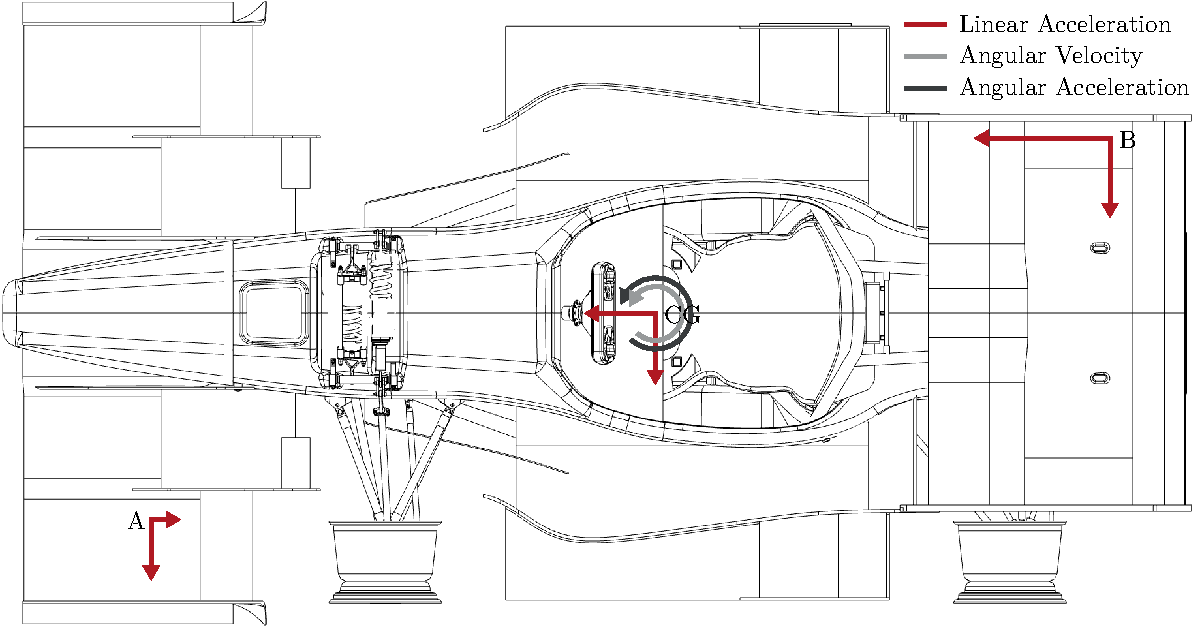
\includegraphics[width=\textwidth]{offcenter_acceleration}%
	\caption{Experienced acceleration at off-center points}
	\label{fig:offcenter-acceleration}
\end{figure}


\subsection{Calculate Angular Acceleration from Linear Acceleration}
Direct measurement of the angular acceleration is often not possible. However, individual components of $\alpha$ can be calculated from the difference of two known linear acceleration vectors at different points $A, B$ with known locations $r^A, r^B$ using equation \ref{eq:angacc-from-linacc-3d}. It is derived from equation \ref{eq:offcenter-acceleration-3d}, with $\Delta a = a^A - a^B$, $\Delta r = r^A - r^B$, and $a^{CG}$ being eliminated by the difference. The points must not be on the rotation axis of the calculated component of $\alpha$, otherwise they experience no angular acceleration. Thus, at least three non-collinear points are required to determine all components of $\alpha$. While the inverse of a cross product is not uniquely determined, as can be seen by the scalar factor $t$, $t = 0$ works well in practice.

\begin{equation}\label{eq:angacc-from-linacc-3d}%
\Delta a = \alpha \times \Delta r + \omega \times (\omega \times \Delta r) \implies%
\alpha = \frac{\Delta r \times (\Delta a - \omega \times (\omega \times \Delta r))}{\norm{\Delta r}^2} + t \cdot \Delta r, t \in \mathbb{R}%
\end{equation}

In two dimensions, this becomes easier to understand. Calculation of the yaw acceleration from the longitudinal and lateral accelerations of two points is shown in equation \ref{eq:angacc-from-linacc-2d}. We can see that the accelerations and distances from different axes are being correlated. The equation even shows how positioning both points on the $z$-axis would result in a zero division, which shows that points off the rotation axis are required. When $A$ and $B$ are directly in front of and behind the \gls{cog} on the $x$-axis so $\Delta r_y = 0$, the equation simplifies to $\ddot{\psi} = \frac{\Delta a_y}{\Delta r_x}$. For practical applications, increasing the distance between the two points minimizes the effects of measurement uncertainty in the result.

\begin{equation}\label{eq:angacc-from-linacc-2d}%
\alpha%
= \frac{\begin{bmatrix}\Delta r_x \\ \Delta r_y \\ 0\end{bmatrix} \times \left(\begin{bmatrix}\Delta a_x \\ \Delta a_y \\ 0\end{bmatrix} - \begin{bmatrix}-\dot{\psi}^2 \cdot r_x \\ -\dot{\psi}^2 \cdot r_y \\ 0\end{bmatrix}\right)}{\begin{Vmatrix}\Delta r_x \\ \Delta r_y \\ 0\end{Vmatrix}^2}%
\implies =\ddot{\psi} = \frac{\Delta r_x\Delta a_y - \Delta r_y\Delta a_x}{\Delta r_x^2 + \Delta r_y^2}%
\end{equation}


\subsection{Transformation of Velocity Between Coordinate Systems}
Most sensor measurements are done in the vehicle coordinate system. Others, such as position measurements from a \gls{gnss} (e.g., \gls{gps}, Galileo, GLONASS), will be made in earth-fixed coordinates, however. To relate these, we need to be able to transform the vehicle velocity from the vehicle coordinate system to the earth-fixed coordinate system, which has an inertial (i.e. non-accelerating) reference frame. Equation \ref{eq:transform-linear-velocity} shows, how this can be achieved by a simple rotation using the heading $\psi$. A two-dimensional treatment is sufficient, since \gls{gnss} altitude information are not relevant here. The transformation extracts the east-/northward components of the local velocities and adds them.

% For EKF position--velocity
\begin{equation}\label{eq:transform-linear-velocity}%
\begin{bmatrix}\prescript{E}{}{v}_x \\ \prescript{E}{}{v}_y\end{bmatrix}%
=\begin{bmatrix}cos(\psi) & -sin(\psi) \\ sin(\psi) & cos(\psi)\end{bmatrix}%
\begin{bmatrix}\prescript{V}{}{v}_x \\ \prescript{V}{}{v}_y\end{bmatrix}%
\end{equation}


\subsection{Components of Vehicle Acceleration}
The motion of a rigid body in the earth-fixed reference frame can be understood as a composition of a rotation and a translation, in our case with the \gls{cog} as center of rotation. In vehicles, this rotation results from cornering.  The acceleration as experienced in the \gls{cog} is the result of the direct linear acceleration and the centripetal force resulting from the rotation, as shown in equation \ref{eq:cornering-acceleration}~\cite[p.~146]{Milliken.1996}. Other than in equation \ref{eq:offcenter-acceleration-3d}, the radius $R$ is not the distance to the \gls{cog} but the corner/curve radius. Since $R$ is usually not known, we can get rid of it using $R = v_{\perp} / \dot{\psi}$ with the tangential velocity $v_{\perp}$.

\begin{subequations}\label{eq:cornering-acceleration}
\begin{alignat}{3}%
a_x &= \dot{v}_x - \dot{\psi}^2 R &= \dot{v}_x - \dot{\psi}v_y \\%
a_y &= \dot{v}_y + \dot{\psi}^2 R &= \dot{v}_y + \dot{\psi}v_x%
\end{alignat}
\end{subequations}


\subsection{Velocity Estimation from Motor Speeds}
While there is a plethora of methods for measuring vehicle velocity, such as optical cross-correlation, radar, 5\textsuperscript{th} wheel and \gls{gnss}, most of them are too expensive for widespread use. Therefore, velocity estimation in many automotive applications is based mainly on motor or wheel speed measurements, which are readily available, especially in electric cars. Equation \ref{eq:wheelspeeds} shows arguably the simplest method to estimate the longitudinal velocity, involving only the dynamic tire radius $r_{dyn}$, the wheel speed $\omega_{wheel}$, the motor speed $\omega_{motor}$ and the motor-to-wheel ratio $i_{gear}$.

\begin{equation}\label{eq:wheelspeeds}%
v_x = \omega_{wheel} r_{dyn} = \frac{\omega_{motor}}{i_{gear}} r_{dyn}%
\end{equation}

This method can only be used for a crude approximation of the longitudinal velocity component. It falls short when the wheel slip, i.e. the relative motion of tire and road surface, increases or in the most severe case even locks up. While the previously mentioned methods are infeasible in most cases, they can be used as ground truth to evaluate estimation methods.

A simple improvement is averaging over all four wheels. More advanced methods are presented in~\cite{Song.2002}. For transient maneuvers with high slip, wheel speed data can be augmented with acceleration measurements. The authors present three approaches. The first estimator uses equation \ref{eq:wheelspeeds} until a high-slip situation occurs, at which point acceleration measurements are integrated over time with the last wheel-based velocity as initial condition. The second estimator reduces noise through a Kalman filter which averages both measurements, weighted by a constant obtained with fuzzy logic. Finally, the third estimator reduces adverse effects of acceleration bias and an incorrect dynamic roll radius through regression.


\section{Estimation Algorithms}
Obtaining the true state of some physical system is next to impossible. Any sensor measurement contains noise and other errors, which distract from the underlying process. Therefore, the challenge is discerning errors from the true value. This is known as \textit{filtering problem}, where we want to obtain the best estimate $\hat{x}_k$ of the system state $x_k$ at time step $k$ based on past observations $z_i, i \leq k$~\cite[p.~67]{Mitter.1996}. Usually, this involves the fusion of multiple sensors and physical models. In this section we explore common estimation methods to solve the filtering problem problem. We will regard their discrete-time instead of their continuous-time versions, since digital observations are based on sampling with a finite rate.

\subsection{Extended Kalman Filter}
The Kalman filter~\cite{Kalman.1960} is the most widely used estimation algorithm~\cite[p.~401]{Julier.2004}. First developed for trajectory estimation in the Apollo space program, it now finds application in most vehicles, aircraft, spacecraft, but even in finance and econometrics. The Kalman filter assumes a linear system, which is often not the case, or only true in a small region of the full range. Therefore, a non-linear version based on the same ideas has been developed with the \gls{ekf}, which we will regard in this section.

The idea of the \gls{ekf} is simple yet powerful: we observe the physical system through noisy measurements but predict the state with a mathematical model of the system. At every time step, we fuse the observations with the predictions based on our confidence in either, basically resulting in a weighted average. For example, a noisy measurement is rather unreliable, while models can never capture all nuances and uncertainties. The fusion yields a good estimate of the true state of the system, better than only measurements or predictions could alone.

The model describes the \textit{state} $x_k$ of the system at time $k$. For example, a train on a track can be described by its position and velocity which are related, so the state is two-dimensional. How the state evolves over time according to a process is shown in the \textit{process equation} \ref{eq:ekf-process-equation}. The process function $f(x_{k-1}, u_k)$ propagates the previous state $x_{k-1}$ and is controlled by external inputs $u_k$, e.g., the train engine accelerating the train, and disturbed process noise $w_k$, which represents unmodeled behavior, e.g., air resistance or friction. The process noise is assumed to be Gaussian with zero mean and a diagonal covariance matrix $Q_k$, i.e no noise terms are correlated.
\begin{equation}\label{eq:ekf-process-equation}%
x_k = f(x_{k-1}, u_k) + w_k%
\end{equation}

While the state is inherent to the system, it can not be directly observed. Rather, we have \textit{observations} $z_k$. The elements of $z_k$ and $x_k$ must not necessarily coincide, i.e. the observation space and state space can differ; for example, we might have multiple observations of the train's velocity but none of the position. The measurement is described by the \textit{measurement equation} \ref{eq:ekf-measurement-equation}. The measurement function $h(x_k)$ gives the observation vector which is disturbed by measurement noise, e.g., resulting from the sensor itself or transmission errors. The measurement noise is assumed to be Gaussian with zero mean and a diagonal covariance matrix $R_k$. We use the measurement equation to be able to fuse real measurements with pseudo-measurements from our model.
\begin{equation}\label{eq:ekf-measurement-equation}%
z_k = h(x_k) + v_k%
\end{equation}

The process and measurements equations acknowledge, that the state can only be modeled and observed with some degree of uncertainty. Therefore, in addition to the state estimate $\hat{x}_k$, we want to keep track of its covariance $P_k$, which is zero mean as well. Together with linearizations, this assumption allows the \gls{ekf} to be much more computationally efficient than more generally applicable algorithms like the particle filter.

The \gls{ekf} algorithm~\cite[p.~16~ff.]{Haykin.2001} is recursive, with each iteration comprising a prediction step and a correction step, i.e. the previous state is first propagated to the current time step using the model and then corrected with the measurements from the real system. In the following description of the algorithm, we distinguish between the predicted state estimate $\hat{x}_k^-$ and covariance $P_k^-$, and the corrected state estimate $\hat{x}_k^+$ and covariance $P_k^+$.

\begin{description}
\item[Prediction] At the beginning of every iteration, the previous corrected state is propagated using the process function to predict the current state (equation \ref{eq:ekf-state-propagation}). Note that the prediction only depends on the directly previous state, not any other states in the history, revealing that the \gls{ekf} assumes an underlying Markov process.
\begin{equation}\label{eq:ekf-state-propagation}%
\hat{x}_k^- = f(\hat{x}_{k-1}^+, u_k)%
\end{equation}

The previous covariance also needs to be propagated, since the estimate uncertainty might change with every step (equation \ref{eq:ekf-cov-propagation}). The Jacobian matrix $F_k$ of the process function, which can be though of as a vector derivative, needs to be evaluated for this step (equation \ref{eq:ekf-process-jacobian}). Additionally, the process noise needs to be accounted for model mismatches, since there are always aspects of the real-world which cannot be modeled. Therefore, leveraging the additive property of Gaussian noise, the process covariance $Q_k$ is added to the propagated covariance.
\begin{align}\label{eq:ekf-cov-propagation}%
P_k^- &= F_k P_{k-1} F_k^T + Q_k \\%
\label{eq:ekf-process-jacobian}%
F_k &= \left. \frac{\partial f}{\partial x} \right|_{x = \hat{x}_{k-1}^+}%
\end{align}

The measurement function then generates pseudo-measurements from the estimated state (equation \ref{eq:ekf-pseudomeasurement}).
\begin{equation}\label{eq:ekf-pseudomeasurement}%
\hat{z}_k = h(\hat{x}_k^-)%
\end{equation}


\item[Correction] Once the prediction has been made, it can be corrected with observations obtained from the real system by taking a weighted average of both. The weighting is determined by the \textit{Kalman gain} $K_k \in [0, 1]$ (equation \ref{eq:ekf-kalman-gain}), which also maps back from the observation space into the state space using the Jacobian matrix $H_k$ of the measurement function (equation \ref{eq:ekf-measurement-jacobian}). The Kalman gain is defined as the ratio of the state-innovation covariance $P_{xy}$ to the innovation covariance $P_{yy}$, and so it captures the uncertainty in the measurements and the model prediction. When the measurement covariance $R_k$ is small relative to the model covariance, the Kalman gain is high and so the measurement is weighted more. On the other hand, when the measurement noise is high, the Kalman gain approaches zero and the model prediction is weighted more.
\begin{align}\label{eq:ekf-kalman-gain}%
K_k &= \underbrace{P_k^- H_k^T}_\textrm{$P_{xy}$} {\underbrace{(H_k P_k^- H_k^T + R_k)}_\textrm{$P_{yy}$}}^{-1} \\%
\label{eq:ekf-measurement-jacobian}%
H_k &= \left. \frac{\partial h}{\partial x} \right|_{x = \hat{x}_{k}^-}%
\end{align}

In the best case, the model and the measurements coincide. However, this is usually not the case, so the real measurements $z_k$ and the pseudo-measurements $\hat{z}_k$ differ, resulting in an \textit{innovation} $y_k$, also called \textit{residual}. The absolute innovation is higher when there is a larger mismatch between the model and the real system. The Kalman gain now determines, how much of the residual is used to correct the prediction. The posterior state estimate $\hat{x}_k^+$ is the final, best estimate for the iteration $k$ and will be used in the next time step (equation \ref{eq:ekf-state-correction}).
\begin{equation}\label{eq:ekf-state-correction}%
\hat{x}_k^+ = \hat{x}_k^- + K(\underbrace{z_k - \hat{z}_k}_\textrm{$y_k$})%
\end{equation}

Additionally, the covariance matrix needs to be updated to account for the correction (equation \ref{eq:ekf-cov-correction}). The covariance is reduced based on the Kalman gain, signifying how the certainty in our estimate has increased by the correction.
\begin{equation}\label{eq:ekf-cov-correction}%
P_k^+ = (I - K H_k)P_k^-%
\end{equation}
\end{description}


\subsection{Unscented Kalman Filter}
While the \gls{ekf} has been successfully applied to problems for a long time, it suffers a number of limitations~\cite[p.~402]{Julier.2004}:
\begin{itemize}
\item The error propagation in equation \ref{eq:ekf-cov-propagation} is only reliably if the linearization in form of the Jacobian matrix $F_k$ is sufficiently accurate. This might not be the case in highly non-linear systems or under the wrong initial estimate. In the worst case, the estimate might even diverge.
\item Linearization can only be applied to differentiable functions, i.e. processes for which a Jacobian exists. Discontinuities and singularities might exist in some cases, making differentiation impossible.
\item The derivation of Jacobian matrices can be very difficult and error-prone for complex systems, both the equations themselves and the conversion to code.
\end{itemize}
Therefore, alternatives to the \gls{ekf} have been developed. A promising algorithm is the \gls{ukf}~\cite{SimonJ.Julier.1997}.

At the core of the \gls{ukf}'s improvement relies on the \gls{ut}. This transformation is a method to approximate the properties of a statistical distribution undergoing a non-linear transformation.

Through the use of the \gls{ut}, linearization of the Jacobian is rendered unnecessary, which aids the filter's stability in non-linear systems. Furthermore, no manual derivation of derivatives is necessary. Still, the performance is equal or better than the \gls{ekf}.
% TODO disadvantages


\section{Outlier Detection}
The quality of the estimate produces by the estimation algorithm is limited by the quality of its input data, especially if the algorithm is not robust. In practice, sensor data can contain anomalous sensor samples, also called \textit{outliers}. While these samples might actually reflect reality, they usually stem from errors during measurement or transmission. In this section, the term \textit{outlier} will refer to bad samples that should be discarded, not surprising but correct samples which can occur in random processes. The challenge is to discern these two while minimizing the number of false positives (leads to discarding good measurements) and false negatives (degrades estimate quality). This improves estimation quality and can be crucial in safety-critical applications. This section presents common outlier types and methods to detect them.


\subsection{Outlier Types}
Outliers can be the result of a variety of issues. For example, heavy vibration and shocks might cause acceleration spikes and an optical cross-correlation sensor might see a featureless surface, so the recognized velocity drops to zero. In cabled transmission, a physical connection might be defect, while in radio transmission, the signal might drop out temporarily or there might be electromagnetic interference. Possible causes can vary a lot between environments, but a highly dynamic environment with many mechanical and electric parts such as an electric race car is likely to produce outliers at some point.

% TODO generate 4 plots and create subfigures
Outliers can be classified in three broad categories~\cites[p.~19]{Kabzan.2019}[p.~165~ff.]{Himmelblau.1994}:
\begin{itemize}
\item Spike/intermittent noise: a transient deviation from previous samples
\item Level shift: a transient deviation of the mean value
\item Drift/spurious trends: a slow variation of the mean value over time
\item Null/signal dropout: not receiving input or zero
\end{itemize}
Drift often occurs as the result of integrating a biased signal, e.g., caused by low frequency noise or temperature changes. While there are other cases of poor data quality such as clipping and excessive noise, they rather stem from calibration problems and hardware errors, so they are not regarded further.

Outliers can be temporary or persistent. While spikes are inherently temporary, outliers of the other three categories might or might not return to normal. For example, a \gls{gps} signal can drop out because the sensor has no satellite connectivity for a couple of seconds but then recovers, while another sensor can be permanently damaged and will not recover. Persistent but not transient outliers are hard to detect, and especially spurious trends cannot easily be distinguished from real trends by their nature. This motivates the need for two separate methods, an approach that is also employed by~\cite{Kabzan.2019}:
\begin{itemize}
\item A simple but strict method for transient outliers
\item A complex but lenient method for persistent outliers
\end{itemize}
With this dual approach false negatives for easy-to-detect transient outliers can be minimized while false positives for hard-to-discern persistent outliers can be avoided.


\subsection{Rudimentary Methods}
Arguably the simplest method is the range check, shown in equation \ref{eq:outlier-range}. A plausible interval $[\tau_{min}, \tau_{max}]$ of values is defined in advance, and if the measurement $z$ is outside of that range, it is marked as outlier. For example, a speed of \SI{200}{\meter\per\second} is highly unlikely for a race car, and also high negative speeds are implausible.
\begin{equation}\label{eq:outlier-range}%
\tau_{min} < z < \tau_{max}%
\end{equation}

Another rudimentary method for detecting spikes is the difference of consecutive samples $z_t, z_{t-1}$, shown in equation \ref{eq:outlier-maxchangerate}. When the difference is higher than the maximum plausible change rate $\tau$, the current measurement is marked as outlier.
\begin{equation}\label{eq:outlier-maxchangerate}%
\abs{z_t - z_{t-1}} < \tau%
\end{equation}

Performing a sanity check is a good first approach to detect gross outliers. However, the thresholds should be set rather high to avoid false positives.


\subsection{Statistical Methods}
Methods based on the statistical properties of a signal can provide more granular checks than the previous rudimentary methods. One of the simplest robust statistics is the median, i.e. the center value when sorting a list of values, which is used in the method shown in equation \ref{eq:outlier-median}~\cite[p.~142]{Basu.2007}. An expected value $\tilde{z}_t$ is calculated using both the median of the last $k$ samples and the median of the differences of the last $k+1$ samples. If the difference between the expected and the actual value exceeds the threshold, the current sample is marked as outlier.
\begin{equation}\label{eq:outlier-median}%
\abs*{z_t - \underbrace{median(z_{t-k}, \ldots, z_{t-1}) + k \cdot median(z_{t-k} - z_{t-k-1}, \ldots, z_{t-1} - z_{t-2})}_\textrm{$\tilde{z}_t$}} < \tau%
\end{equation}

If an \gls{ekf} is used, a chi-squared test can be used to detect anomalies based on the residuals, as shown in equation \ref{eq:outlier-chisquared}~\cites[p.~4292]{Hausman.2016}[p.~2050~f.]{Valls.2018}. Since the residual $y$ is Gaussian distributed with the innovation covariance matrix $P_{yy}$ (for nomenclature, refer to section \ref{sec:background-ekf}), the normalized sum of squares of the residual values should be distributed according to a chi-squared distribution $\chi^2$ with as many degrees of freedom as there are measurements. An outlier is detected when the chi-squared test at a significance level of $\tau$ failed.
\begin{subequations}\label{eq:outlier-chisquared}
\begin{alignat}{2}%
y &= z - h(\hat{x}^-) \\%
P_{yy} &= H P^- H^T + R \\%
r^T P_{yy}^{-1} r &< \chi^2(\tau)%
\end{alignat}
\end{subequations}

Drift detection becomes easier when multiple sensors measure the same variable and can be compared. A simple variance-based approach based on this idea is shown in equation \ref{eq:outlier-variance}~\cite[p.~20]{Kabzan.2019}. For each time step, the summed variance of $n$ sensors is calculated, based on the mean $\mu_z$ of their measurements at that instant. Once the threshold $\tau \in (0, 1)$ is exceeded, the measurement with the highest contribution to the summed variance is marked as outlier.
\begin{equation}\label{eq:outlier-variance}%
\sum_{i=1}^n (z_i - \mu_z)^2 < \tau%
\end{equation}



EKF bank
describe distinction between fault detection and isolation

